%%%%%%%%%%%%%%%%%%%%%%%%%%%%%%%%%%%%%%%%%
% Beamer Presentation
% LaTeX Template
% Version 1.0 (10/11/12)
%
% This template has been downloaded from:
% http://www.LaTeXTemplates.com
%
% License:
% CC BY-NC-SA 3.0 (http://creativecommons.org/licenses/by-nc-sa/3.0/)
%
%%%%%%%%%%%%%%%%%%%%%%%%%%%%%%%%%%%%%%%%%

%----------------------------------------------------------------------------------------
%	PACKAGES AND THEMES
%----------------------------------------------------------------------------------------

\documentclass{beamer}

\mode<presentation> {

% The Beamer class comes with a number of default slide themes
% which change the colors and layouts of slides. Below this is a list
% of all the themes, uncomment each in turn to see what they look like.

%\usetheme{default}
%\usetheme{AnnArbor}
%\usetheme{Antibes}
%\usetheme{Bergen}
%\usetheme{Berkeley}
%\usetheme{Berlin}
%\usetheme{Boadilla}
%\usetheme{CambridgeUS}
%\usetheme{Copenhagen}
%\usetheme{Darmstadt}
%\usetheme{Dresden}
%\usetheme{Frankfurt}
%\usetheme{Goettingen}
%\usetheme{Hannover}
%\usetheme{Ilmenau}
%\usetheme{JuanLesPins}
%\usetheme{Luebeck}
\usetheme{Madrid}
%\usetheme{Malmoe}
%\usetheme{Marburg}
%\usetheme{Montpellier}
%\usetheme{PaloAlto}
%\usetheme{Pittsburgh}
%\usetheme{Rochester}
%\usetheme{Singapore}
%\usetheme{Szeged}
%\usetheme{Warsaw}


% As well as themes, the Beamer class has a number of color themes
% for any slide theme. Uncomment each of these in turn to see how it
% changes the colors of your current slide theme.

%\usecolortheme{albatross}
%\usecolortheme{beaver}
%\usecolortheme{beetle}
%\usecolortheme{crane}
%\usecolortheme{dolphin}
%\usecolortheme{dove}
%\usecolortheme{fly}
%\usecolortheme{lily}
%\usecolortheme{orchid}
%\usecolortheme{rose}
%\usecolortheme{seagull}
%\usecolortheme{seahorse}
%\usecolortheme{whale}
%\usecolortheme{wolverine}

%\setbeamertemplate{footline} % To remove the footer line in all slides uncomment this line
%\setbeamertemplate{footline}[page number] % To replace the footer line in all slides with a simple slide count uncomment this line

%\setbeamertemplate{navigation symbols}{} % To remove the navigation symbols from the bottom of all slides uncomment this line
\setbeamertemplate{caption}[numbered]
}

\usepackage{graphicx} % Allows including images
\usepackage{booktabs} % Allows the use of \toprule, \midrule and \bottomrule in tables
\usepackage{epstopdf,epsfig}
\usepackage{amsmath}
\usepackage[english]{babel}
\usepackage{lmodern}
\usepackage[utf8]{inputenc}

%----------------------------------------------------------------------------------------
%	TITLE PAGE
%----------------------------------------------------------------------------------------

\title{A Multi-Objective Genetic Algorithm for Evaluating Build Order Effectiveness in Starcraft~II} % The short title appears at the bottom of every slide, the full title is only on the title page

\author{Jonas Schmitt} % Your name
\date{\today} % Date, can be changed to a custom date

\AtBeginSection[]
{
 \begin{frame}
 \frametitle{Overview}
 \tableofcontents[currentsection]
 \end{frame}
}

\begin{document}

\begin{frame}
\titlepage % Print the title page as the first slide
\end{frame}

%\begin{frame}
%\frametitle{Outline} % Table of contents slide, comment this block out to remove it
%\tableofcontents % Throughout your presentation, if you choose to use \section{} and \subsection{} commands, these will automatically be printed on this slide as an overview of your presentation
%\end{frame}
%------------------------------------------------
\section{Motivation}
\begin{frame}{Starcraft II}
\begin{columns}[c] % the "c" option specifies center vertical alignment
    \column{.5\textwidth} % column designated by a command
    \begin{itemize}
		\item Military science-fiction real-time strategy game
		\item \alert{Goal:} Producing the right combination of units (\alert{Macromanagement}) to destroy the other player's units and structures in combat (\alert{Micromanagement})
	\end{itemize}
    \column{.5\textwidth}
    	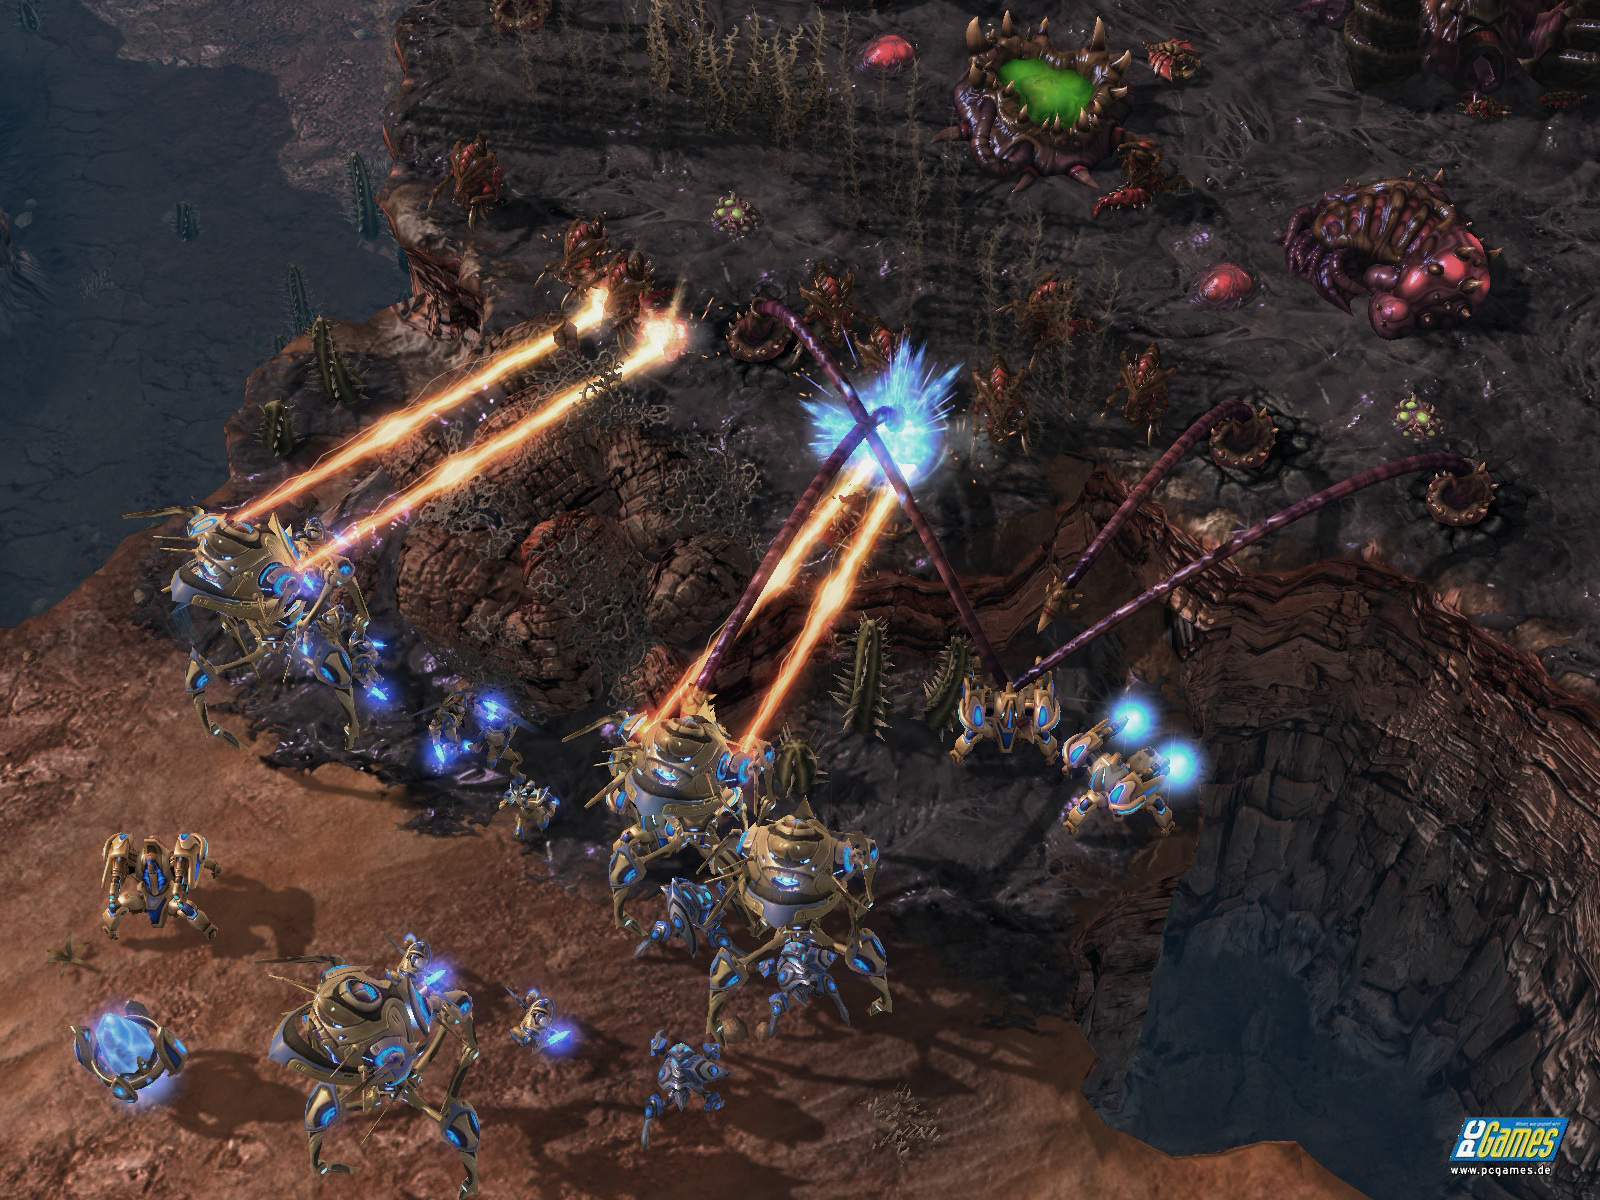
\includegraphics[width=1.0\linewidth]{starcraft-2-screenshot.jpg}
\end{columns}
\begin{itemize}
\item E-Sport scene with growing popularity (price pools up to US\$170,000)
\\ $\Rightarrow$ Importance of \alert{Balancing} (Are all three races equally strong?) 
\end{itemize}
\end{frame}

\begin{frame}{Balancing}
\begin{itemize}
\item \alert{Macromanagement:} Which units can be produced in a certain amount of time?
\\ $\Rightarrow$ `` A Multi-objective Genetic Algorithm for Build Order Optimization in StarCraft II '' by Harald Köstler and Björn Gmeiner
\item \alert{Micromanagement:} Is it possible to predict which of two groups of units wins in combat?
\\ $\Rightarrow$ No suitable approach for Starcraft II yet
\end{itemize}
\end{frame}

\begin{frame}{Evaluation of Micromanagement}
\begin{itemize}
\item \alert{Input:} Build Order, i.e. the list of units that have been produced until a certain point of time in the game
\item \alert{Goal:} Simulate and optimize the behavior (moving and attacking) of each single unit
\\ $\Rightarrow$ It can be predicted which player would succeed in a combat assuming optimal control
\end{itemize}
\end{frame}

\section{Forward Simulation}
\begin{frame}{Forward Simulation}
    \begin{itemize}
\item No freely available API for controlling units in the game directly
\\ $\Rightarrow$ An efficient forward simulation is required that determines the winner of an encounter based on a finite set of parameters
\item \alert{Idea:} Describe the behavior of each unit by a number of parametrized \alert{Potential Fields}
\item[$\Rightarrow$] Units create multiple artificial potential fields around their position which are modeled as linear functions
\end{itemize}
\end{frame}

\begin{frame}{Potential Fields}
\begin{columns}[c] % the "c" option specifies center vertical alignment
    \column{.5\textwidth} % column designated by a command
\begin{figure}[h]
	%\centering
	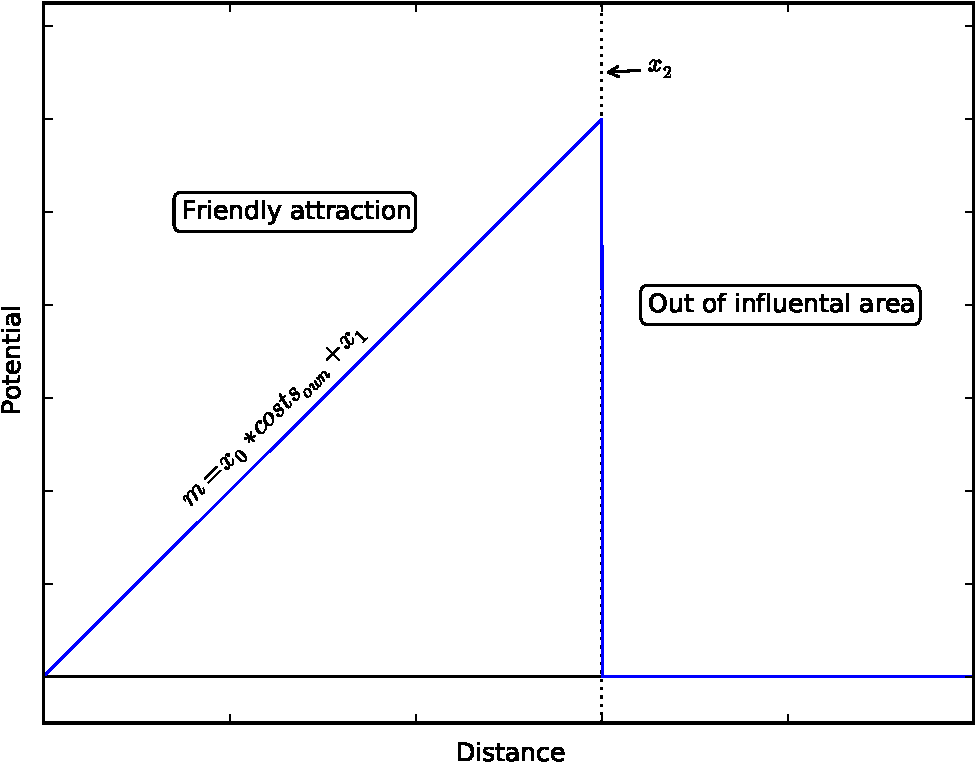
\includegraphics[width=1.0\linewidth]{friend-crop.pdf}
	\caption{Attractive potential of friendly units.}
	\label{fig:graph_friend}
\end{figure}
    \column{.5\textwidth}
\begin{figure}[h]
	%\centering
	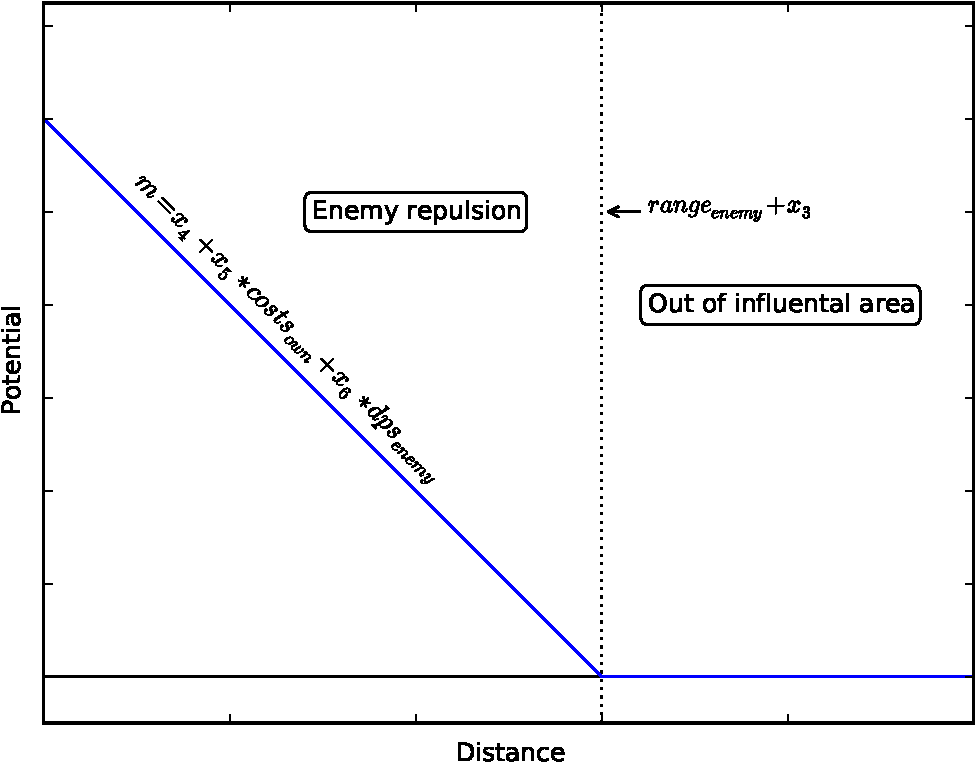
\includegraphics[width=1.0\linewidth]{enemy1-crop.pdf}
	\caption{Repulsive potential of enemy units.}
	\label{fig:graph_enemy1}
\end{figure}
\end{columns}
\end{frame}

\begin{frame}{Potential Fields}
\begin{center}
\begin{figure}[h]
	%\centering
	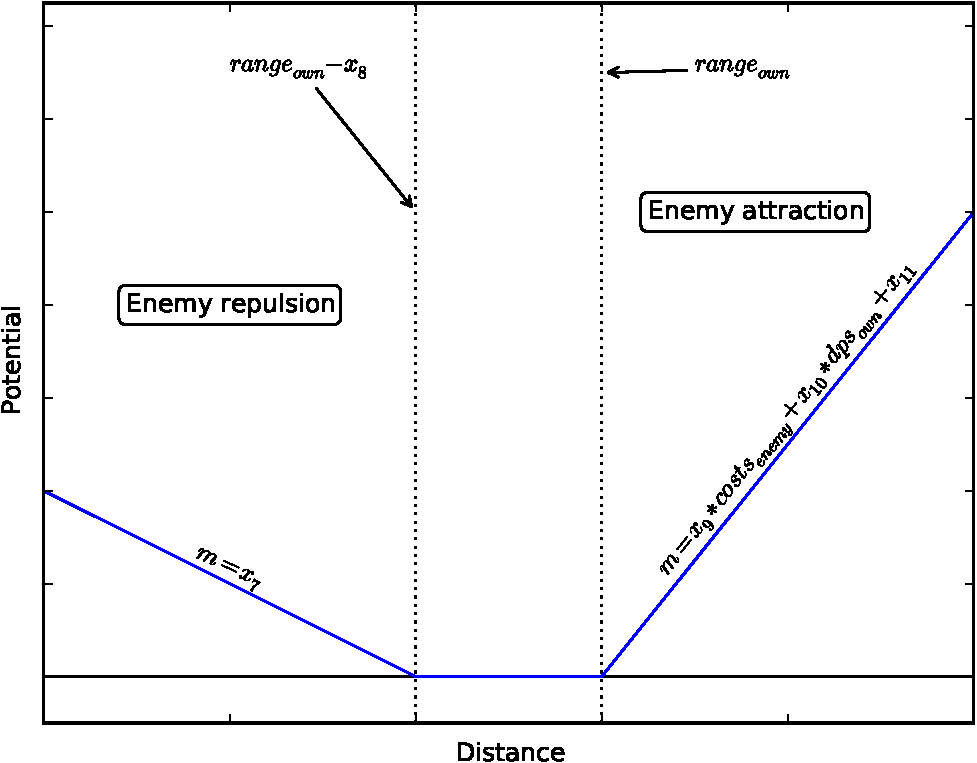
\includegraphics[width=0.5\linewidth]{enemy2-crop.pdf}
	\caption{Attractive potential of enemy units.}
	\label{fig:graph_enemy2}
\end{figure}
\end{center}
\end{frame}
\begin{frame}{Forward Simulation}
During a time step the following actions are performed by each unit:
\begin{itemize}
\item If \alert{attacking} is possible, a target is chosen among all enemies within attack range by favoring units that can be defeated, prioritized by the amount of applicable damage
\item Else, the unit \alert{moves} and its position at the next time step is computed with the following equation:
	\begin{equation*}
		\vec{p_{i+1}} = \vec{p_i} +\vec{F} \times s
	\end{equation*}
	where $\vec{p_i}$ is the position at time step $i$, $\vec{F}$ the current force and $s$ the movement range. 
\end{itemize}
\end{frame}

\begin{frame}{Forward Simulation}
\begin{itemize}
\item The \alert{force} of each unit is recomputed after a fixed number of time steps by accumulating the gradients of all potential fields applying to it:
	\begin{equation*}
		\vec{F} = \sum_{j=1}^n \vec{F}_j
	\end{equation*}
	where $n$ is the number of potential fields affecting the unit and $\vec{F}_j$ the gradient of the $j$th potential field
\item The forward simulation finishes when either all units of a player have been defeated or the simulation’s duration exceeds a certain limit.
\end{itemize}
\end{frame}

\section{Optimization}
\begin{frame}{Optimization}
\begin{itemize}
\item \alert{Goal:} Iteratively optimize the parameters for both opponents' units against each other
\item \alert{Challenges:} 
\begin{itemize}
\item Large search space (at least 14 real valued parameters for each different type of unit) 
\item No knowledge about the relationship between in- and output
\end{itemize}
\item[$\Rightarrow$] \alert{Genetic Algorithms} are suitable search heuristics for problems of this type
\end{itemize}
\end{frame}

\begin{frame}{Optimization}
\alert{Overview}
\begin{itemize}
\item Encode the parameters of both opponents
\item Choose suitable starting values for the optimization objective (strategy used by the opponent) for both populations
\item Replace the objectives every $n$ generation by the respective optima and reevaluate both populations
\item The obtained results can be used to evaluate the effectiveness of both build orders against the respective other one
\end{itemize}
\end{frame}

\begin{frame}{Single-Objective Genetic Algorithm}

\begin{itemize}
\item The fitness of each individual is approximated with a simple formula:  \\
\begin{equation*}
\begin{split}
\text{Fitness} & = \text{total applied damage} + \text{total remaining health} 
\\ & + \text{value of killed units} + \text{value of remaining units} 
\end{split}
\end{equation*}
\item[$\Rightarrow$] Determine the \alert{optimal combination of genetic operators} for the computational costlier multi-objective optimization
\end{itemize}
\end{frame}

\begin{frame}{Multi-Objective Genetic Algorithm}
\begin{itemize}
\item Considers all relevant objectives (applied damage, remaining health, value of units killed, value of units remaining etc.) independently to achieve a better spread of solutions
\item Based on \alert{nondominated sorting} (NSGA-II)
\item[$\Rightarrow$] Perform the actual optimization with suitable operators to \alert{evaluate the effectiveness of certain build orders} compared to each other
\end{itemize}
\end{frame}

\section{Results}

\begin{frame}{Results}

\begin{itemize}
\item Measuring the Performance of different Combinations of common Genetic Operators (Selection, Crossover and Mutation Methods) for the single-objective genetic algorithm
\item \alert{Online Performance:} Average fitness of all evaluations
\item \alert{Offline Performance:} Average fitness of the optima of each generation
\item Parameters used: 
\end{itemize}
\centering
\begin{tabular}{c | c | c | c | c }
Population & Iterations & Generations & Mutation\\
Size & & per Iteration & Probability \\
\hline \hline
500 & 100 & 10 & 1 \%
\end{tabular}

\end{frame}

\begin{frame}{Results}
\begin{table}
\begin{tabular}{c | c | c | c | c }
Selection & Crossover & Mutation & Online Performance \\
\hline \hline
RWS & NPC & IM & 82.17 \\
SUS & SPC & IM & 80.64 \\
RWS & TPC & RM & 79.19 \\
RWS & UC & RM & 79.12 \\
SUS & SPC & BFM & 79.04
\end{tabular}
\caption{Online Performance}
\end{table}

SUS: Stochastic Universal Sampling, RWS: Roulette Wheel Selection, TS: Tournament Selection (Binary) \\
SPC: Single-Point Crossover, TPC: Two-Point Crossover, NPC: N-Point-Crossover (with $n=\frac{1}{2}$ number of parameters), UC: Uniform Crossover \\
BFM: Bit-Flip Mutation, IM: Interchanging Mutation, RM: Reversing Mutation

\end{frame}


\begin{frame}{Results}
\begin{table}
\begin{tabular}{c | c | c | c | c }
Selection & Crossover & Mutation & Offline Performance \\
\hline
SUS & SPC & IM & 94.50 \\
RWS & NPC & IM & 94.09 \\
RWS & TPC & RM & 93.78 \\
TS & TPC & IM & 93.52 \\
RWS & TPC & IM & 93.48
\end{tabular}
\caption{Offline Performance}
\end{table}


SUS: Stochastic Universal Sampling, RWS: Roulette Wheel Selection, TS: Tournament Selection (Binary) \\
SPC: Single-Point Crossover, TPC: Two-Point Crossover, NPC: N-Point-Crossover (with $N=\frac{1}{2}$ number of parameters), UC: Uniform Crossover \\
BFM: Bit-Flip Mutation, IM: Interchanging Mutation, RM: Reversing Mutation

\end{frame}



%\begin{frame}{Task scheduling in concurrent computer environments}
%Optimization goals:
%\begin{itemize}
%	\item[1)] Equally distribute the workload over the available processors 
%	\item[2)] Minimize the communication between them 
%\end{itemize}
%\vspace*{0.5cm}
%Can be formulated as Graph Partitioning problem:
%%Graph partitioning for use in concurrent computer environments
%\begin{itemize}
%	\item[1)] \textcolor{red}{Vertices} represent \textcolor{red}{computational} costs \\
%	\item[2)] \textcolor{blue}{Edges} represent \textcolor{blue}{communication} costs \\
%\end{itemize}
%\end{frame}




%\section{References}
%\begin{frame}
%\frametitle{References}
%\footnotesize{
%\begin{thebibliography}{99} % Beamer does not support BibTeX so references must be inserted manually as below
%
%\input{biblio}
%
%%\bibitem[Smith, 2012]{p1} John Smith (2012)
%%\newblock Title of the publication
%%\newblock \emph{Journal Name} 12(3), 45 -- 678.
%\end{thebibliography}
%}
%\end{frame}

%------------------------------------------------

\begin{frame}
\Huge{\centerline{Thank you for the attention!}}
\end{frame}

%----------------------------------------------------------------------------------------

\end{document}
